%************************************************
\chapter{Results}\label{ch:results}
%************************************************
In this chapter, the learning performance and regularization behavior of the ALIF, STDP-ALIF, and Izhikevich neurons are compared.
Then, the effect of stacking multiple recurrent layers on the learning performance and speed is examined.
Figure \ref{fig:inoutpair} shows a typical classification result of a full validation sentence.

	\begin{figure}[ht]
	    \myfloatalign
	    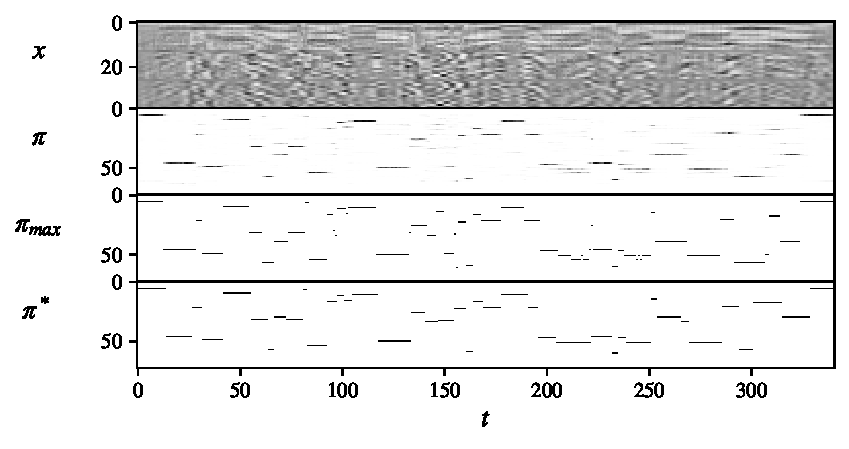
\includegraphics[width=\linewidth]{gfx/InOutPair}
	    \caption[Input/output/target example]{An example validation result using a trained ALIF model. The plot in the top row shows the standardized MFCC frames including its first and second derivatives of a sentence changing over time. The plot in the second row shows the probability distributions $\pi$ of the frame-wise outputs of the model. The plot in the third row indicates the predicted phone $\pi_\text{max}$ per frame. The plot in the last row shows the target phones $\pi^*$.}
	    \label{fig:inoutpair}
	  \end{figure}

\section{Comparing neuron models}
	\paragraph{Accuracy}
		The main outcome of the neuron model comparison is that in these results, the Izhikevich neuron type performs poorly compared to the ALIF and STDP-ALIF neuron models.
		In Figure \ref{fig:percwrong} the Izhikevich neuron reaches a misclassification rate of 93.8\% on the test set, which is only slightly better than constantly guessing the most frequent class.
		The ALIF neuron model reaches a test misclassification rate of 58.4\% in relatively few iterations, after which validation performance starts to decrease.
		The STDP-ALIF neuron model scores best, reaching a performance of 48.3\% after approximately 3500 iterations.
		Note that the test performance was obtained from the model with the best validation accuracy (the used hyperparameters are listed in Table \ref{tab:hparams}).

		Figure \ref{fig:crossentropy} illustrates the decrease of the cross-entropy score, which for the ALIF and STDP-ALIF neurons is comparable to that of the misclassification rate.
		The cross-entropy and classification performance of the Izhikevich neuron stalls relatively quickly at poor levels, suggesting that it trains its bias toward more frequent phone classes in the training data rather than learning a general relationship between input MFCCs and classes.

		\begin{figure}[bth]
		    \myfloatalign
		    \subfloat[Percentage of samples wrongly classified.]
		    {\label{fig:percwrong}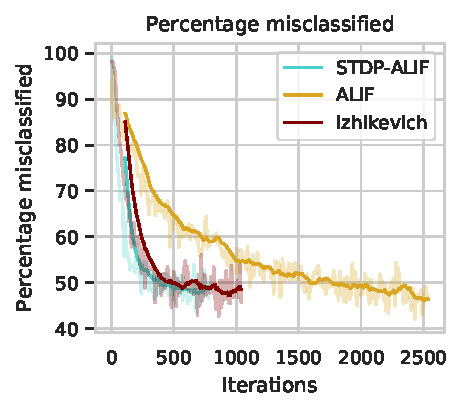
\includegraphics[height=5cm, keepaspectratio]{gfx/percwrong}} \quad
		    \subfloat[Cross-entropy loss (log-scaled).]
		    {\label{fig:crossentropy}%
		        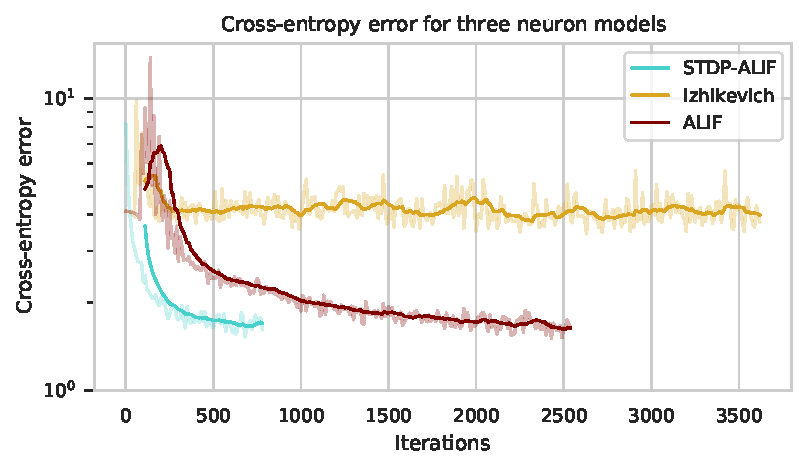
\includegraphics[height=5cm, keepaspectratio]{gfx/crossentropy}}
		    \caption[Single-layer classification performance per neuron model]{Classification performance on the validation data for each of the three neuron models in a single-layer e-prop model. The opaque lines indicate the running average of the real validation scores indicated by the transparent lines. The star symbols indicate the performances on the test set, with a misclassification rate of 93.5\% for the Izhikevich neuron, 58.4\% for the ALIF neuron, and 48.3\% for the STDP-ALIF neuron type.}\label{fig:sl-acc}
		\end{figure}

	\paragraph{Firing rate}
		Figure \ref{fig:freqs} illustrates the effect of the firing regularization term.
		It can be observed that the ALIF and STDP-ALIF neuron models are able to quickly modulate their mean spiking frequencies to the desired target frequency of \SI{10}{\Hz}, but the Izhikevich neuron overshoots to a mean spiking frequency of approximately \SI{18}{\Hz}.

		Figure \ref{fig:regerr} illustrates the decrease of the regularization error.
		The regularization error of the Izhikevich and ALIF neuron models quickly converges to fluctuate around a constant value, whereas that of the STDP-ALIF neuron model continues to decrease over time, even after the mean spiking frequency and classification performance have both converged to a plateau.

		\begin{figure}[bth]
		    \myfloatalign
		    \subfloat[Mean spiking frequency. Note the logarithmic horizontal axis.]
		    {\label{fig:freqs}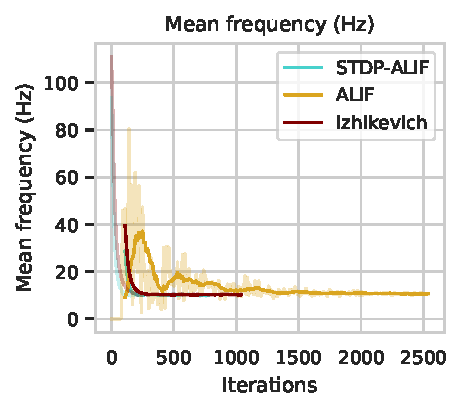
\includegraphics[height=5cm, keepaspectratio]{gfx/hz}} \quad
		    \subfloat[Regularization error. Note the logarithmic vertical axis.]
		    {\label{fig:regerr}%
		        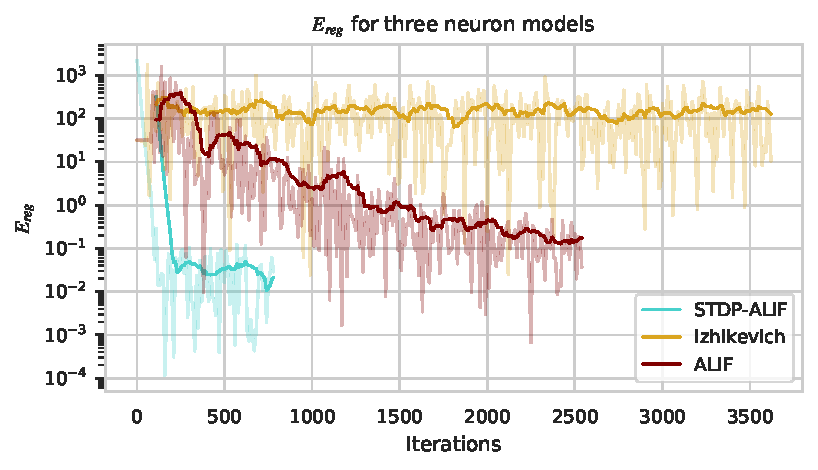
\includegraphics[height=5cm, keepaspectratio]{gfx/regerr}}
		    \caption[Single-layer firing rate regularization per neuron model]{Effect of firing rate regularization on the validation data for each of the three neuron models.}\label{fig:sl-reg}
		\end{figure}

\section{Comparing network depth}
The comparison between the network depth in Figures \ref{fig:ml-pwrong-alif}--\ref{fig:ml-pwrong-izh} suggests that single-layer e-prop networks train considerably more efficiently and accurately than multi-layer e-prop networks and show less variance among validation runs.
This holds for all tested neuron types.
The cross-entropy error, spiking frequency, and regularization error are also better for single-layer networks (see Figure \ref{fig:ml-otherresults}).

\begin{figure}[bth]
    \myfloatalign
    \subfloat[ALIF model.]
    {\label{fig:ml-pwrong-alif}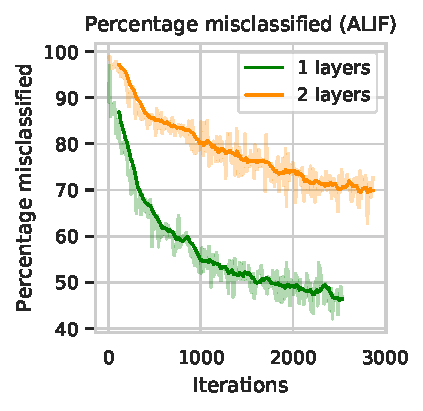
\includegraphics[height=5cm, keepaspectratio]{gfx/ml-percwrong-ALIF}} \quad
    \subfloat[STDP-ALIF model.]
    {\label{fig:ml-pwrong-stdpalif}%
        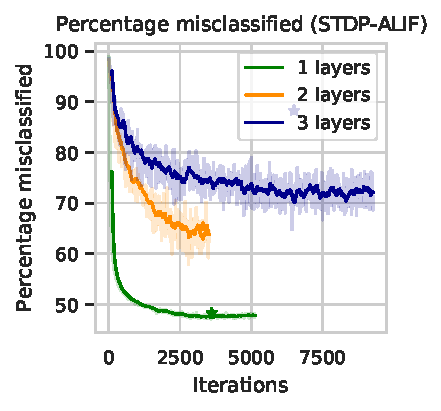
\includegraphics[height=5cm, keepaspectratio]{gfx/ml-percwrong-STDP-ALIF}} \\
    \subfloat[Izhikevich model.]
    {\label{fig:ml-pwrong-izh}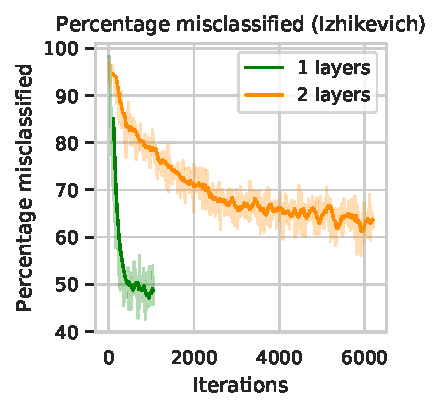
\includegraphics[height=5cm, keepaspectratio]{gfx/ml-percwrong-Izhikevich}}
    \caption[Single- and multi-layer accuracy comparison]{Accuracy comparison on the validation data between single- and multi-layer e-prop models.}\label{fig:ml-percwrong}
\end{figure}
